\begin{frame}{Annexes}
    {Context}

    \begin{block}{Multi-Agent Systems (MAS) paradigm for complex \& distributed problems}
        \begin{itemize}
            \item \textbf{task decomposition}: missions delegated to agents achieved through cooperation~\cite{Raileanu2023};
            \item \textbf{benefits}: handle conflicting goals, parallel computation, system robustness, scalability\dots
        \end{itemize}
    \end{block}

    \begin{block}{\textbf{Organization}: key for MAS designing}
        \begin{itemize}
            \item \textbf{coordination}: how to collaboratively achieve a common goal~\cite{Hubner2007};
            \item \textbf{dynamic \& uncertain environments}: flexible runtime behavior to adapt~\cite{Kathleen2020};
        \end{itemize}
    \end{block}

    \begin{block}{Methods and practice for MAS design}
        \begin{itemize}
            \item \textbf{approach + organizational model}: methods rely on designers' experience to hand-craft agents' \textbf{policies} so resulting MAS achieve goals;
                  %   \begin{itemize}
                  %       \item Examples: \emph{GAIA}~\cite{Wooldridge2000,Cernuzzi2014}, \emph{ADELFE}~\cite{Mefteh2015}, or \emph{DIAMOND}~\cite{Jamont2015}, \emph{KB-ORG}~\cite{Sims2008}
                  %   \end{itemize}
            \item \textbf{simulation to reality}: 1) safe \& efficient MAS design in high fidelity simulated environment; \quad 2) transfer to real environment to perform adequately~\cite{Schon2021}.
        \end{itemize}
        \vspace{1ex}
        \quad $\Longrightarrow$ \textbf{Iterative process proceeding by trial and error}

    \end{block}

\end{frame}

\begin{frame}{Annexes}
    {MAS basics}

    \begin{block}{Keywords}
        \begin{itemize}
            \item \textbf{Agent}: entity immersed in an environment perceiving observation and making decision autonomously to achieve some goals;
            \item \textbf{MAS}: a set of agents collaborating with self/re-organizing mechanisms to achieve their goal;
            \item \textbf{Organization}: the agents' interactions even though it may be implicit;
            \item \textbf{Organizational Model (OM)}: medium to formally describe an explicit/implicit organization;
            \item \textbf{Organizational Specifications (OS)}: components of an OM to characterize an organization
        \end{itemize}
    \end{block}

    \begin{block}{Organizational model: $\mathcal{M}OISE^+$}
        \begin{itemize}
            \item more complex than \emph{Agent Group Roles} (integration of standards);
            \item takes into account the social aspects between agents explicitly;
            \item possible to link agents' policies to organizational specifications.
        \end{itemize}
    \end{block}

\end{frame}

\begin{frame}{Annexes}
    {MARL basics}

    \begin{block}{Keywords}
        \begin{itemize}
            \item \textbf{Policy}: the \textquote{logic} to choose next action according to observation for an agent;
            \item \textbf{History/trajectory}: the tuple of (observation, action) couples over an episode;
            \item \textbf{Joint-policy / Joint-history}: all of the agents' policies / histories as tuples;
            \item \textbf{Reinforcement learning}: an agent updates its policy to maximize a cumulative reward;
            \item \textbf{Multi-Agent Reinforcement Learning (MARL)}: extends to multiple agents that learn while considering the actions of other agents;
        \end{itemize}
    \end{block}

\end{frame}

\begin{frame}{Annexes}{AOMEA approach: Overview}

    \begin{columns}

        \begin{column}{0.6\textwidth}

            \textbf{Phase 1: Modeling}

            \begin{itemize}
                \item Manually develop a simulated environment ($1.1$) where agents must cooperate to achieve goal ($1.2$);
                \item Can define expected roles behavior as histories;
                \item May constraint agents to roles ($1.3$).
            \end{itemize}

        \end{column}

        \begin{column}{0.4\textwidth}
            \centering
            \adjustbox{trim={0.\width} {0.82\height} {0.\width} {0.\height}, clip}{%
                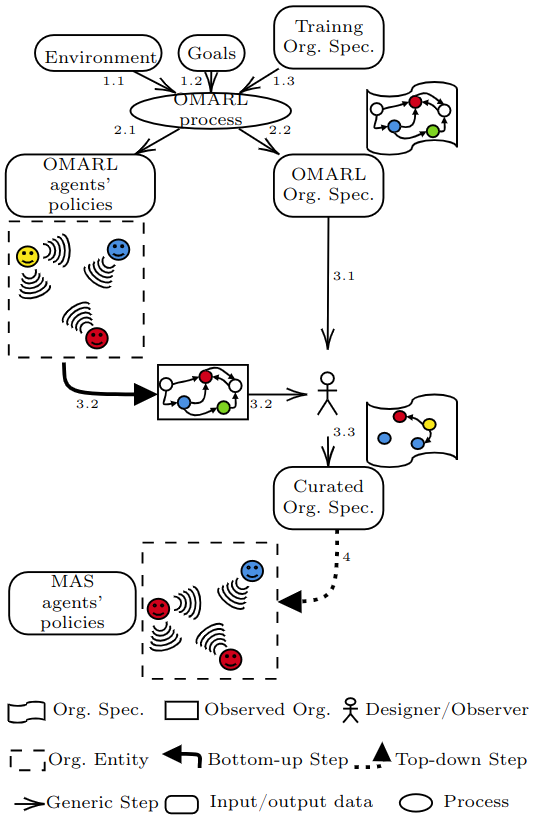
\includegraphics[width=1.2\linewidth]{figures/AOMEA_illustrative_view}
            }
        \end{column}

    \end{columns}

\end{frame}


\begin{frame}{Annexes}{AOMEA approach: Overview}

    \begin{columns}

        \begin{column}{0.6\textwidth}

            \textbf{Phase 2: Solving}

            \begin{itemize}
                \item Organization-oriented MARL (OMARL) algorithm: MARL process augmented with Organizational model;
                \item Solve satisfying constrained roles' histories ($2.1$);
                \item Gets associated OS ($2.2$)
            \end{itemize}

        \end{column}

        \begin{column}{0.4\textwidth}
            \centering
            \adjustbox{trim={0.\width} {0.56\height} {0.\width} {0.\height}, clip}{%
                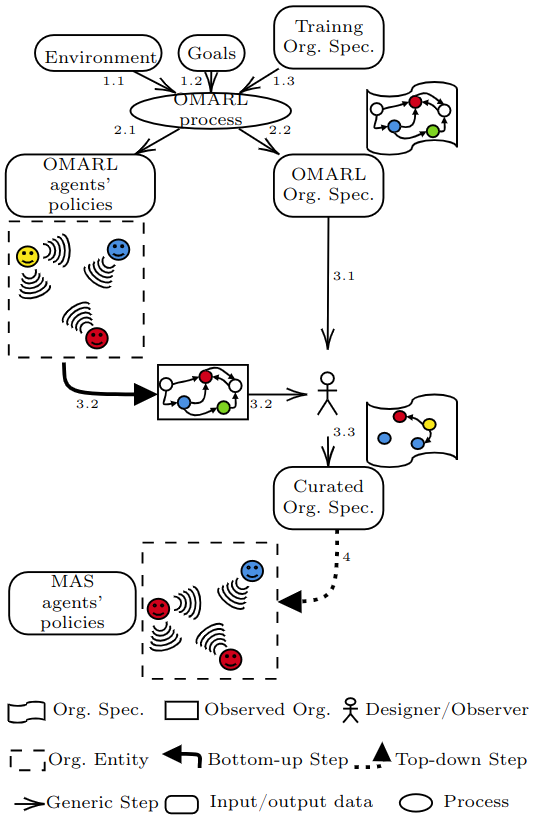
\includegraphics[width=1.2\linewidth]{figures/AOMEA_illustrative_view}
            }
        \end{column}

    \end{columns}


\end{frame}

\begin{frame}{Annexes}{AOMEA approach: Overview}

    \begin{columns}

        \begin{column}{0.6\textwidth}

            \textbf{Phase 3: Analyzing}

            \begin{itemize}
                \item Designers observe the trained agents' policies ($3.2$);
                \item Designers observe the computed OS ($3.1$): understand how they reach the goal;
                \item Designers get some design indications for a MAS to achieve the goal: curated OS ($3.3$).
            \end{itemize}


        \end{column}

        \begin{column}{0.4\textwidth}
            \centering
            \adjustbox{trim={0.\width} {0.35\height} {0.\width} {0.188\height}, clip}{%
                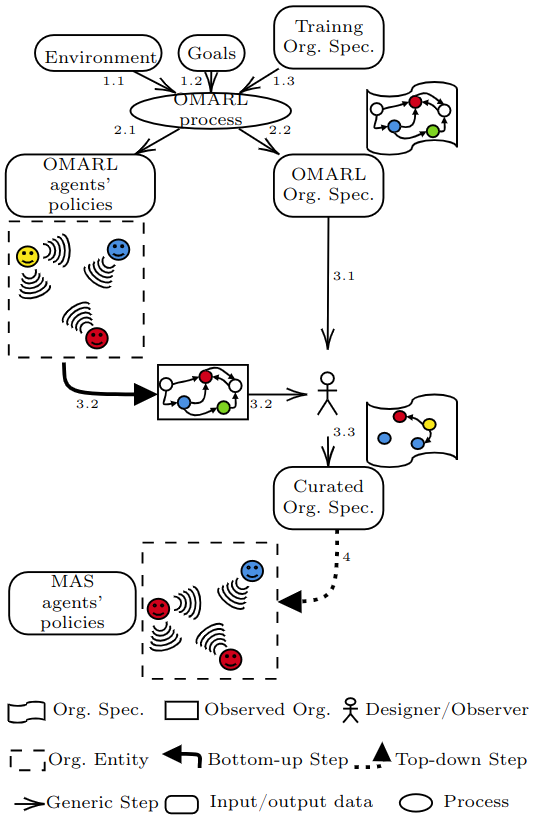
\includegraphics[width=1.2\linewidth]{figures/AOMEA_illustrative_view}
            }
        \end{column}

    \end{columns}

\end{frame}

\begin{frame}{Annexes}{AOMEA approach: Overview}

    \begin{columns}

        \begin{column}{0.6\textwidth}

            \textbf{Phase 4: Developing}

            \begin{itemize}
                \item Designers observe the curated OS for implementing a MAS;
                \item Regular MAS development hence addressing safety issues;
                \item Implemented MAS assessed in simulations.
            \end{itemize}

        \end{column}

        \begin{column}{0.4\textwidth}
            \centering
            \adjustbox{trim={0.\width} {0.15\height} {0.\width} {0.57\height}, clip}{%
                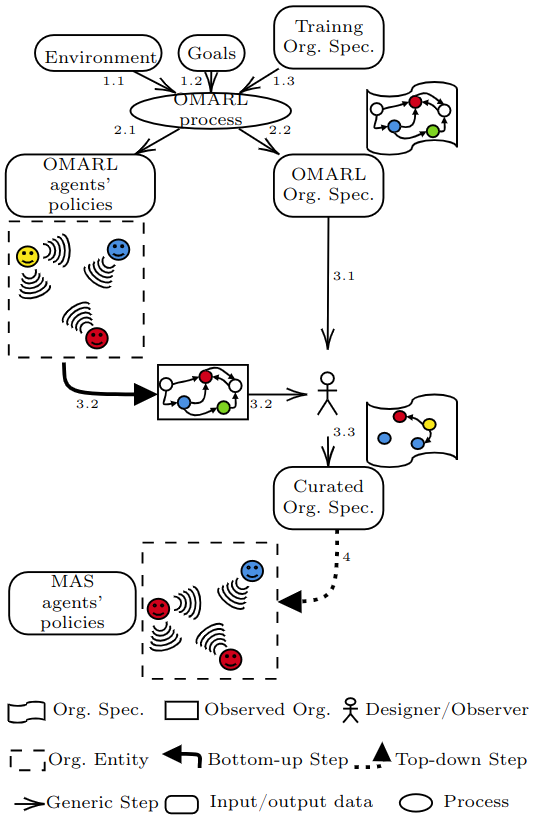
\includegraphics[width=1.2\linewidth]{figures/AOMEA_illustrative_view}
            }
        \end{column}

    \end{columns}

\end{frame}



\begin{frame}{Annexes}{AOMEA approach: Theoretical core}

    \begin{block}{Organization-oriented MARL (OMARL)}
        An MARL process augmented with an OM for:
        \begin{itemize}
            \item \textbf{Constraining Policies Space}: gets the joint-policies satisfying the given design specifications;
            \item \textbf{Inferring Organizational Specifications}: gets the specifications from the agents' policies.
        \end{itemize}

    \end{block}

    \begin{block}{\emph{Partial Relations with Agent History and Organization Model} algorithm (PRAHOM)}
        Implementing an OMARL process\dots
        \begin{enumerate}
            \item \textbf{Constraining Policies Space}
                  \begin{itemize}
                      \item Cannot use policies directly $\rightarrow$ \textbf{histories} characterizing \textbf{policies};
                      \item Relations between \textbf{OS} to expected \textbf{histories};
                      \item Agents constrained to OS $\rightarrow$ at each step: available actions updated regarding \textbf{OS} histories.
                  \end{itemize}

            \item \textbf{Inferring Organizational Specifications}
                  \begin{itemize}
                      \item Analyze histories $\rightarrow$ characterize collective behaviors as OS;
                      \item Using known relations between OS and histories;
                      \item Using general OS definition regarding histories.
                  \end{itemize}
        \end{enumerate}
    \end{block}
\end{frame}

\begin{frame}{Annexes}{AOMEA approach: Theoretical core}

    \textbf{Constraining Policies Space} during training

    \begin{columns}

        \begin{column}{0.3\textwidth}

            \begin{itemize}
                \item At each step, available actions set is changed to match policy constraints defined by users;
                \item Constraints integrated through: external correction, learning, internal policy change.
            \end{itemize}

        \end{column}

        \begin{column}{0.8\textwidth}
            \begin{figure}
                \centering
                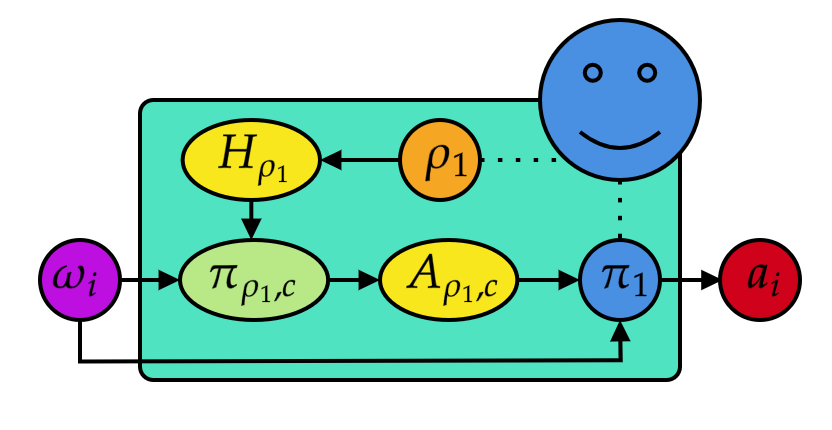
\includegraphics[width=0.7\linewidth]{figures/prahom_training_constrain.png}
                \caption*{A summary view of the PRAHOM constraining}
                \label{fig:prahom_process}
            \end{figure}
        \end{column}

    \end{columns}

\end{frame}


\begin{frame}{Annexes}{AOMEA approach: Theoretical core}

    \textbf{Inferring Organizational Specifications}

    \begin{columns}

        \begin{column}{0.3\textwidth}

            \begin{itemize}
                \item \textbf{Knowledge-based Organizational Specifications Identification (KOSIA)}
                \item \textbf{General Organizational Specifications Infererence (GOSIA)}
            \end{itemize}

        \end{column}

        \begin{column}{0.8\textwidth}
            \begin{figure}
                \centering
                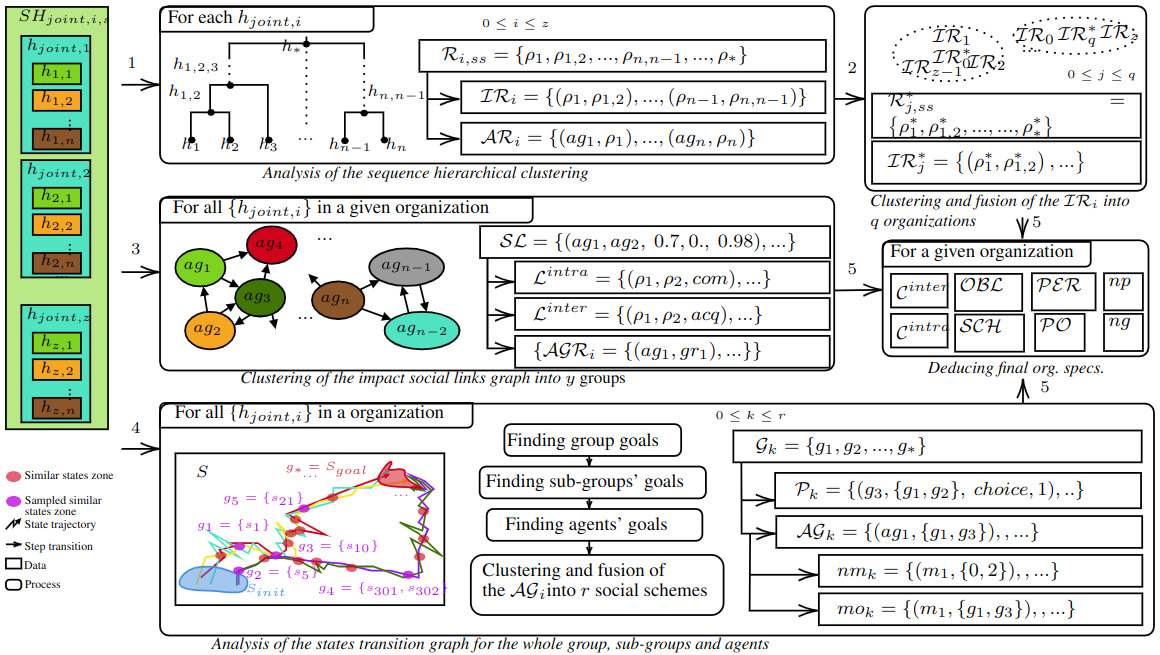
\includegraphics[width=0.95\linewidth]{figures/GOSIA_view.png}
                \caption*{A summary view of the GOSIA process}
                \label{fig:gosia_process}
            \end{figure}
        \end{column}

    \end{columns}

\end{frame}
